\documentclass[tikz,border=10pt,multi]{standalone}
\usetikzlibrary{decorations.pathmorphing,calc}

\newsavebox{\videoin}
\savebox{\videoin}{%
  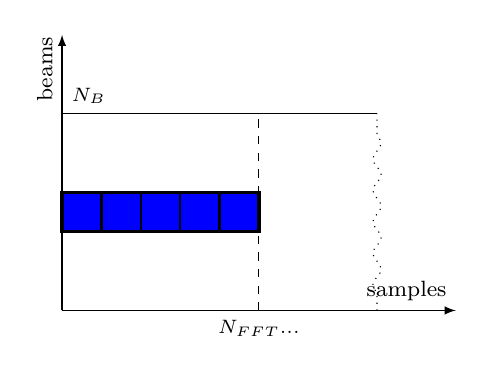
\begin{tikzpicture}[scale=.5,>=latex]
    \coordinate (o) at (0,0,0);
    \draw[->] (o) -- (0,7) node [very near end, above, sloped] {\footnotesize beams};
    \draw[->] (o) -- (10,0) node [very near end, above, sloped] {\footnotesize samples};

    \draw[very thick, fill=blue]
    (5,2) -- (5,3) -- (0,3) -- (0,2) -- cycle
    ;

    \foreach \i in {1,...,4} {
      \draw[thick] (\i,3) -- (\i,2);
    }
    
    \draw(0,5) node[anchor=south west] {\scriptsize $N_B$} -- (8,5);    
    \draw[dashed](5,0) node[anchor=north] {\scriptsize $N_{FFT}...$} -- (5,5);
    
    \draw[dotted,decorate,decoration={snake, segment length=4mm, amplitude=1.5pt,pre length=0.2cm, post length=0.2cm}]
    (8,0) -- (8,5);
  \end{tikzpicture}%
}



\begin{document}
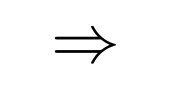
\begin{tikzpicture}
  \node (in) {\usebox{\videoin}};
  \node[anchor=west,xshift=1cm] (out) at (in.east) {\usebox{\videoin}};
  \node[] at ($(in)!.5!(out)$) {\Huge $\Rightarrow$};
\end{tikzpicture}
\end{document}

%%% Local Variables:
%%% mode: latex
%%% TeX-master: t
%%% End:
